\chapter{Methods}

\label{cha:methods}

In this chapter, we describe our implementation of the game Breakthrough and the methods for training a neural network to play the game. The training process uses MCTS, as described in Section \ref{sec:mcts}, to guide its training. We outline the architecture we used for our neural network.

The training algorithm is a reinforcement learning self-play algorithm based on previous work by DeepMind~\cite{silver:alphagozero}.

\section{Game Implementation}

In this section, we will take a look at the implementation of the Breakthrough neural network, how we model its state representation and the pseudo-code for training.

\subsection{Description of the input and output}

For a neural network to be able to use input, that input needs to be numeric. We model the board with a single $N\times M\times 3$ array with two values $\{0,1\}$, where the first two indices on the $z$ axis represent the players, and the last layer on the $z$ axis represents which players turn it is. The first $z$ index represents whites pawns, that is, each $(x,y)$ position on the board where white has a pawn has the value $1$ otherwise it has $0$, and similarily on the second layer for the black player. The last $z$ layer, contains all $1$'s if it is the white players turn otherwise all $0$'s.

One of the outputs of the neural network is the policy vector. The policy vector is a $3$-dimensional matrix where the lengths of the dimensions are $N * M * 6$ and each index of the matrix represents an action moving from cell $x,y$ moving to the direction $z$. The directions are as follows: $0$ represents moving upwards and to the left diagonally on the board, $1$ upwards, $2$ upwards and to the right diagonally, $4$ downwards and to the left diagonally, $5$ downwards, and lastly $6$ downwards and to the right diagonally. The cell values indicate the probability distribution of the search selecting that move. Importantly, before we select a move from the neural networks prediction we zero out the illegal moves, and renormalize the array such that it sums to $1$.

\section{Neural Network Architecture}

The neural network architecture we opted to use was a single convolutional layer with a ReLU\cite{hinton:relu} activation function, followed by 5 residual layers each containing two layers of convolution, batch normalization, and a ReLu activation. Lastly, a split policy/value head, where the output of the last residual layer is split into two different outputs. The policy head are two layers: first a final convolutional layer, and then a fully connected layer with a \textit{log softmax} layer. The value head consists of three layers: first a convolutional layer, then a fully connected layer, and lastly a fully connected layer with a \textit{tanh} activation function. Figure~\ref{fig:nnarch} depicts the architecture. Using this architecture we end up with $1{,}737{,}986$ trainable parameters.

\begin{figure}[]
    \centering

    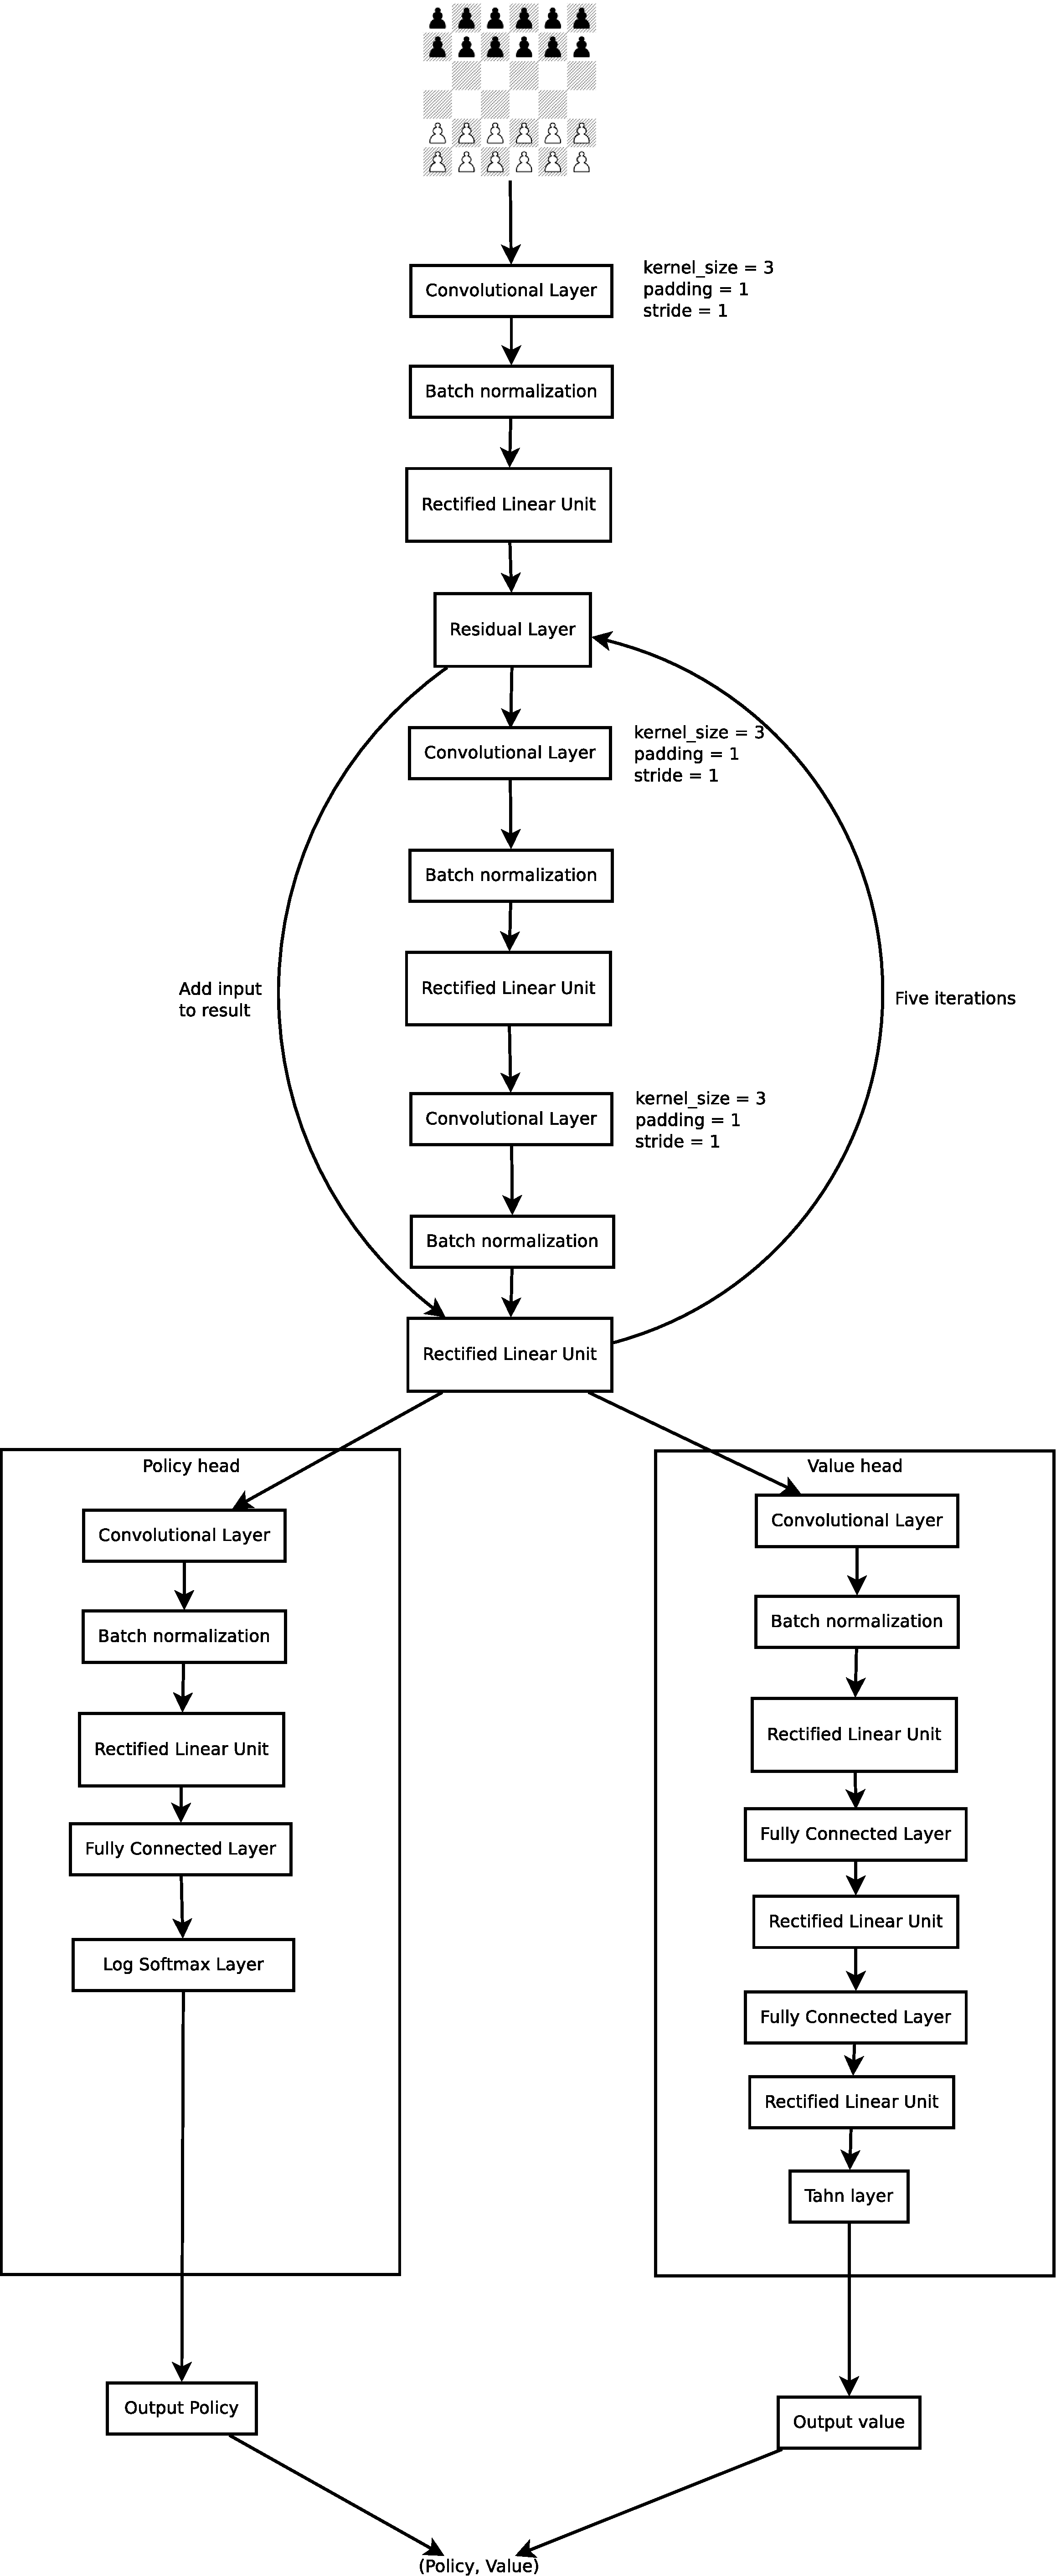
\includegraphics[width=0.65\textwidth]{graphics/test}

    \caption{Neural Network Architecture}
    \label{fig:nnarch}
\end{figure}

\subsection{Convolutional Layers}

It is important to understand why we use convolutional layers when dealing with board games as convolution is more typically associated with an image. This is because a convolutional layer is focused on merging multiple input parameters to a single neuron, making it an input parameter for the next layer representing the locality around the center point of the original input. Playing the game of Breakthrough, a piece is only able to capture pieces in its immediate vicinity. This lead to the selection of a $3$-d convolutional kernel with a size of $3x3$ and a stride of $1$.

We require a global view of the board. This is why we use multiple residual layers with convolution. These residual layers stack convolutions on each other making the final convolution represent the locality of all the other localities, allowing the neural network to have a representation of the whole game state in its parameters. The selection of parameters was done for these reasons as well as to most closely resemble the architecture described in AlphaZero\cite{Silver:alphazero}.

\subsection{Residual Layers}

The residual layers add the output of the previous layer and the results of the residual layer. On a higher level, this leads to the internal representation of the neural network to maintain the whole game boards in its representation, s.t. two areas that are far away from each other maintain the same level of locality as two that are close.

The reason for why we use a residual layer for applying a convolution layer multiple times is to gain locality of the whole game board. A residual layer applies a function like this $res(x) = x + l(x)$ where $x$ is the input and $l(x)$ is the function of the layer, commonly a convolutional layer.

\subsection{Policy Head}

The policy head of the neural network returns a vector of the size of the action space $w * h * 6$ where $w$ is the width of the board, $h$ is the height of the board, and $6$ represents the six cardinal direction pawns can move (straight, and diagonally both left and right for the first player, and backward for the second player). The vector is then masked s.t. the values representing moves that can not be played on the board are given the value of $0$.

\subsection{Value Head}

The value head of the neural network returns a single value representing the predicted value of the neural network. This predicted value is trained to be the end value of the game after taking the predicted move.

\section{Implementation}

This subsection focuses on the implementation of the various functions required to train the neural network to play Breakthrough. The description is mainly through pseudo-code, and the code is available on GitHub for examination~\cite{siggi:github}.

\subsection{Self-play}

\begin{algorithm}[t]
    \caption{Neural network self-play pseudo-code}
    \label{alg:selfplay}
    \begin{algorithmic}[1]
        \STATE \textbf{neural network} nn1 = randomizedInitialNN()
        \STATE \textbf{neural network} nn2 = randomizedInitialNN()
        \WHILE{\TRUE}
        \STATE{dataset = \textbf{generate\_dataset}(nn1)}
        \STATE{nn1.train\_on\_examples(dataset)}
        \STATE{win\_rate = \textbf{compete}(nn1,nn2)}
        \IF{win\_rate > $0.5$}
        \STATE{nn2 = nn1.copy()}
        \ELSE
        \STATE{nn1 = nn2.copy()}
        \ENDIF
        \STATE \textbf{save}(nn1)
        \ENDWHILE
    \end{algorithmic}
\end{algorithm}

To train the neural network to play Breakthrough we initialize two neural networks nn1 and nn2 with random weights. Then we let nn1 play against itself using MCTS with PUCT to select moves. We collect data from this self-play to train on. The data collected is $(s, \pi, \tau, p, v)$, where $s$ is the state, $\pi$ is the action policy vector provided by MCTS with PUCT, $\tau$ the end reward for the episode $1$ if white wins, $-1$ if black wins. $p$ is the policy vector predicted by the neural network, and $v$ is the predicted reward of the game by the neural network.

The pseudo-code is shown as Algorithm~\ref{alg:selfplay}.

\subsection{Compete}

\begin{algorithm}[t]
    \caption{Neural network compete pseudo-code}
    \label{alg:competition}
    \begin{algorithmic}[1]
        \STATE{\textbf{Input:} neural network nn1, neural network nn2}
        \STATE{\textbf{Output:} win rate for white player}
        \STATE{white\_wins $= 0$}
        \STATE{game = \textbf{initial\_breakthrough}()}
        \FOR{1 \TO 100}
        \WHILE{\textbf{not} game.is\_terminal()}
        \STATE{nn1.make\_move()}
        \STATE{nn2.make\_move()}
        \ENDWHILE
        \IF{game.white\_wins()}
        \STATE{white\_wins++}
        \ENDIF
        \ENDFOR
        \STATE{\textbf{return} white\_wins/100}
    \end{algorithmic}
\end{algorithm}

The compete function differs from the self-play function in such a way that we select the moves by a single pass through the neural network thereby only evaluating the neural networks ability to predict best actions. The pseudo-code shown as Algorithm~\ref{alg:competition}.

\subsection{Loss Function}

The data collected is backpropagated through the NN moving the weights to the direction of this loss function $l = (p * \pi) + (\tau - v)^2$ for each state the NN encountered during self-play. Importantly the variable $p$ has masked illegal actions to $0$ to direct the NN to not learn on illegal moves.

\section{Explainable State Representations}

In this section we describe the process of training a Concept Activation Vector in order to linearly separate each state into points in a space with the concept and ones without the concept.

\subsection{Testing with Concept Activation Vectors}

Once the neural network has learned to play the game of Breakthrough, we examine its internal state w.r.t HLC's that we understand. The first examined HLC is material advantage, that is, the number of pieces that a player has over the opponent. The higher-level idea to human players would be that they are in a better position since they have more pieces.

\begin{algorithm}[t]
    \caption{CAV creation pseudo-code}
    \label{alg:CAVcreation}
    \begin{algorithmic}[1]
        \STATE{\textbf{Input:} neural network nn, column\_name, breakpoint, data\_set, sample\_size}
        \STATE{\textbf{Output:} A concept activation vector for the column with \textit{column\_name}}
        \STATE{positive\_set = \textbf{select\_positive\_samples}(data\_set, column\_name, sample\_size)}
        \STATE{negative\_set = \textbf{select\_negative\_samples}(data\_set, column\_name, sample\_size)}
        \STATE{labelled\_set = positive\_set + negative\_set}
        \STATE{unlabelled\_set = dataset - unlabelled\_set}
        \STATE{model = \textbf{StochasticGradientDescentClassifier}()}
        \FOR{state \textbf{in} labelled\_set}
        \STATE{//Modify labelled dataset to contain internal representations}
        \STATE{state = nn.\textbf{get\_internal\_representation}(state)}
        \ENDFOR
        \STATE{train\_set, test\_set = \textbf{train\_test\_split}(labelled\_dataset)}
        \STATE{model.\textbf{train}(train\_set)}
        \STATE{prediction\_score, roc\_auc\_score = model.\textbf{predict}(test\_set)}
        \STATE{\textbf{return} model}
    \end{algorithmic}
\end{algorithm}

To examine the higher-level component we take a look at the internal state of the neural network itself. To do this, we take a state, and run it through the neural network, and while the state is propagating through the network we select a layer to split the network, we call that layer $l_{split}$. At that point in time the state is a mutated vector $l_{split}(l_{split-1}(...l_0(state)))$ of the initial state. We save that vector as a point in the N-dimensional space that it represents, and once we've gathered enough points in that N-dimensional space we're able to train a linear classifier using the HLC as a label. We train a Stochastic Gradient Descent classifier, from the SKLearn library, to construct a hyper-plane that splits the space into two binary states, one that contains the HLC and another that doesn't. We show pseudo-code of this process in Algorithm \ref{alg:CAVcreation}.

\begin{figure}[]
    \centering
    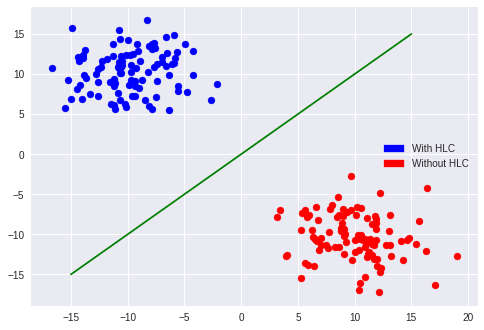
\includegraphics[width=0.7\textwidth]{graphics/linear_separation}
    \caption{Trained linear classifier on a 2-dimensional space}
    \label{fig:scattersplit}
\end{figure}

An example of how this would look with only two dimensions is shown in Figure \ref{fig:scattersplit}. Once we've successfully trained this linear classifier we can run another state $s$ through the neural network. Once the prediction has finished, we view the selected action $a$ of $s$ from the policy vector $p$ from the neural network. We then apply the backpropagation algorithm up to that same layer $l_{split}$ and evaluate the gradient there. If that gradient moves in the direction of the HLC we say that the state includes the HLC, and that it doesn't if the gradient moves away from the HLC.

\begin{figure}[]
    \centering
    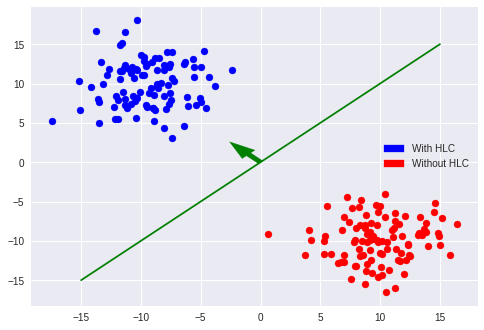
\includegraphics[width=0.7\textwidth]{graphics/linear_separation_with_direction}
    \caption{Trained linear classifier on a 2-dimensional space with arrow representing gradient}
    \label{fig:scattersplitarrow}
\end{figure}

We show an example in Figure \ref{fig:scattersplitarrow}, where the arrow in the image represents the direction the gradient is moving, if it moves toward the HLC the state $s$ includes the HLC otherwise it does not. Using this method we evaluate the internal representation of the state within the neural network and can see whether it recognizes the HLC.

\begin{algorithm}[t]
    \caption{Evaluate a neural network w.r.t concepts pseudo-code}
    \label{alg:CAVapplication}
    \begin{algorithmic}[1]
        \STATE{\textbf{Input:} \textbf{neural network} nn, \textbf{concept activation vector} cav}
        \STATE{\textbf{Output:} Portion of encountered states that contain the concept of the concept activation vector}
        \STATE{state\_count = 0}
        \STATE{has\_tcav = 0}
        \FOR{1 \TO 100}
        \STATE{current\_state = \textbf{Breakthrough}.initial\_state}
        \WHILE{! current\_state.\textbf{terminal}()}
        \STATE{current\_internal\_representation = \\ nn.\textbf{get\_internal\_representation}(current\_state)}
        \STATE{output = nn.\textbf{finish\_propagating}(current\_internal\_representation)}
        \STATE{gradient\_direction = \\ nn.\textbf{get\_gradient}(current\_internal\_representation, output)}
        \STATE{tcav\_score = cav $ \cdot $ gradient\_direction}
        \IF{\textbf{same\_direction}(tcav\_score, cav)}
            \STATE{has\_tcav++}
        \ENDIF
        \STATE{state\_count++}
        \STATE{current\_state = nn.\textbf{get\_next\_state}(current\_state)}
        \ENDWHILE
        \ENDFOR
        \STATE{\textbf{return} has\_tcav / state\_count}
    \end{algorithmic}
\end{algorithm}

In Algorithm \ref{alg:CAVapplication} we show pseudo-code depicting how we evaluate if a neural network recognizes a given concept. The resulting value from running the algorithm is, the proportion of states that the neural network encountered during playing against it self that contain the HLC.


\section{Summary}

In this chapter we described the architecture of the neural network, including how we model Breakthrough to be able to learn to play the game, we described the processes we use to learn from self play. In the following chapter we will evaluate the neural network.
